\documentclass[uplatex]{jsarticle}

\usepackage{amssymb}
\usepackage{amsmath}
\usepackage{mathrsfs}
\usepackage{amsfonts}
\usepackage{mathtools}

\usepackage{xcolor}
\usepackage[dvipdfmx]{graphicx}



\usepackage{ulem}

\usepackage{braket}

%%%%%ハイパーリンク
%\usepackage[colorlinks=true,urlcolor=blue!70!black,citecolor=blue!60!black,linkcolor=blue!60!black]{hyperref}
%\usepackage{aliascnt} %for creating different biblatex references for different theoremstyles
\usepackage[setpagesize=false,dvipdfmx]{hyperref}
\usepackage{aliascnt}
\hypersetup{
    colorlinks=true,
    citecolor=blue,
    linkcolor=blue,
    urlcolor=blue,
}

\renewcommand{\eqref}[1]{\textcolor{blue}{(\ref{#1})}}

%%%%%%ハイパーリンク


%%%%%図式
%\usepackage{tikz}%%%図
\usepackage{amscd}%%%簡単な図式

\usepackage{tikz}
\usepackage{tikz-cd} %commutative diagrams in TikZ
\usetikzlibrary{calc}
\usetikzlibrary{matrix,arrows}
\usetikzlibrary{decorations.markings}

%%%%%図式



%%%%%%%%%%%%定理環境%%%%%%%%%%%%
%%%%%%%%%%%%定理環境%%%%%%%%%%%%
%%%%%%%%%%%%定理環境%%%%%%%%%%%%

\newcommand{\myTheoremEnvironments}[1]{#1}

\usepackage{amsthm}

%%%%%%%%%%%%Plain型%%%%%%%%%%%%

\myTheoremEnvironments{

%%%%%%%%%%%%definition型%%%%%%%%%%%%

\theoremstyle{definition}

\renewcommand{\sectionautorefname}{Section}

\newtheorem{thm}{Theorem}%[section]
\newcommand{\thmautorefname}{Theorem}


\newaliascnt{prop}{thm}%%%カウンター「prop」の定義(thmと同じ)
\newtheorem{prop}[prop]{Proposition}
\aliascntresetthe{prop}
\newcommand{\propautorefname}{Proposition}%%%カウンター名propは「命題」で参照する

\newaliascnt{cor}{thm}
\newtheorem{cor}[cor]{Corollary}
\aliascntresetthe{cor}
\newcommand{\corautorefname}{Corollary}

\newaliascnt{lem}{thm}
\newtheorem{lem}[lem]{Lemma}
\aliascntresetthe{lem}
\newcommand{\lemautorefname}{Lemma}

%%%%%%%アルファベットで番号づける定理環境
\newtheorem{thmA}{Theorem}[section]
\newcommand{\thmAautorefname}{Theorem}
\renewcommand\thethmA{\Alph{thmA}}

\newtheorem{corA}{Theorem}[section]
\newcommand{\corAautorefname}{Corollary}
\renewcommand\thecorA{\Alph{corA}}

\newaliascnt{defi}{thm}
\newtheorem{defi}[defi]{Definition}
\aliascntresetthe{defi}
\newcommand{\defiautorefname}{Definition}

\newaliascnt{rem}{thm}
\newtheorem{rem}[rem]{Remark}
\aliascntresetthe{rem}
\newcommand{\remautorefname}{Remark}

\newaliascnt{reconstruction}{thm}
\newtheorem{reconstruction}[reconstruction]{Reconstruction}
\aliascntresetthe{reconstruction}
\newcommand{\reconstructionautorefname}{Reconstruction}

%%%%%%%番号づけない定理環境
\newtheorem*{exam*}{Example}
\newtheorem*{rrem*}{Remark}
\newtheorem*{defi*}{Definition}
\newtheorem*{setting*}{Setting}

%%%%%%%%%%%%定理環境%%%%%%%%%%%%
%%%%%%%%%%%%定理環境%%%%%%%%%%%%
%%%%%%%%%%%%定理環境%%%%%%%%%%%%
}




%%%%%箇条書き環境
\usepackage[]{enumitem}

\makeatletter
\AddEnumerateCounter{\fnsymbol}{\c@fnsymbol}{9}%%%%fnsymbolという文字をenumerate環境のパラメーターで使えるようにする。
\makeatother

\makeatletter
\renewcommand{\p@enumii}{}
\makeatother

\renewcommand{\theenumi}{(\roman{enumi})}%%%%%itemは(1),(2),(3)で番号付ける。
\renewcommand{\labelenumi}{\theenumi}

\renewcommand{\theenumii}{(\alph{enumii})}%%%%%itemは(1),(2),(3)で番号付ける。
\renewcommand{\labelenumii}{\theenumii}

\usepackage{moreenum}


\makeatletter
\newcommand*{\@yuyuspadecount}[1]{\ensuremath{
\ifcase #1\or\spadesuit\or\spadesuit_2\or\spadesuit_3
\or\spadesuit_4\or\spadesuit_5\or\spadesuit_6
\or\spadesuit_7\or\spadesuit_8\or\spadesuit_9
\else\@ctrerr\fi\relax}}
\newcommand*{\yuyuspadecount}[1]{%
\expandafter\@yuyuspadecount\csname c@#1\endcsname
}
\AddEnumerateCounter{\yuyuspadecount}{\@yuyuspadecount}{9}

\newcommand*{\@yuyuclubcount}[1]{\ensuremath{
\ifcase #1\or\clubsuit_1\or\clubsuit_2\or\clubsuit_3
\or\clubsuit_4\or\clubsuit_5\or\clubsuit_6
\or\clubsuit_7\or\clubsuit_8\or\clubsuit_9
\else\@ctrerr\fi\relax}}
\newcommand*{\yuyuclubcount}[1]{%
\expandafter\@yuyuclubcount\csname c@#1\endcsname
}
\AddEnumerateCounter{\yuyuclubcount}{\@yuyuclubcount}{9}

\newcommand*{\@yuyustarcount}[1]{\ensuremath{
\ifcase #1\or\star_1\or\star_2\or\star_3
\or\star_4\or\star_5\or\star_6
\or\star_7\or\star_8\or\star_9
\else \@ctrerr \fi\relax}}
\newcommand*{\yuyustarcount}[1]{%
\expandafter\@yuyustarcount\csname c@#1\endcsname
}
\AddEnumerateCounter{\yuyustarcount}{\@yuyustarcount}{9}
\makeatother
%%%%%箇条書き環境



\newcommand{\myOriginalPackages}[1]{#1}

\myOriginalPackages{

\usepackage{mandorasymb}
\usepackage{applekeys}
\renewcommand{\qedsymbol}{\pencilkey}
%\renewcommand{\qedsymbol}{\kinoposymbniko}

}



\usepackage{latexsym}

\newcommand{\myMacros}[1]{#1}

\myMacros{
\DeclareMathOperator{\Hom}{Hom}
\DeclareMathOperator{\Isom}{Isom}
\DeclareMathOperator{\ISOM}{\mathbf{Isom}}
\DeclareMathOperator{\id}{\mathrm{id}}
\DeclareMathOperator{\im}{\mathrm{Im}}

\DeclareMathOperator{\coker}{\mathrm{coker}}
\DeclareMathOperator{\colim}{\mathrm{colim}}
\DeclareMathOperator{\plim}{\mathrm{lim}}
\DeclareMathOperator{\rank}{\mathrm{rank}}
\DeclareMathOperator{\codim}{\mathrm{codim}}

\DeclareMathOperator{\Spec}{\mathrm{Spec}}
\DeclareMathOperator{\Proj}{\mathrm{Proj}}
\DeclareMathOperator{\Sym}{\mathrm{Sym}}
\DeclareMathOperator{\Ext}{\mathrm{Ext}}
\DeclareMathOperator{\Bs}{\mathrm{Bs}}
\DeclareMathOperator{\Bl}{\mathrm{Bl}}
\DeclareMathOperator{\Sing}{\mathrm{Sing}}
\DeclareMathOperator{\red}{\mathrm{red}}
\DeclareMathOperator{\Reg}{\mathrm{Reg}}
\DeclareMathOperator{\Ridge}{\mathrm{Ridge}}
\DeclareMathOperator{\Hilb}{\mathrm{Hilb}}
\DeclareMathOperator{\Grass}{\mathrm{Grass}}


\newcommand{\A}{\mathbb{A}}
\newcommand{\C}{\mathbb{C}}
\renewcommand{\P}{\mathbb{P}}
\newcommand{\R}{\mathbb{R}}
\newcommand{\Q}{\mathbb{Q}}
\newcommand{\Z}{\mathbb{Z}}
\newcommand{\N}{\mathbb{N}}



\newcommand{\mcA}{\mathcal{A}}
\newcommand{\mcB}{\mathcal{B}}
\newcommand{\mcC}{\mathcal{C}}
\newcommand{\mcD}{\mathcal{D}}
\newcommand{\mcE}{\mathcal{E}}
\newcommand{\mcF}{\mathcal{F}}
\newcommand{\mcG}{\mathcal{G}}
\newcommand{\mcH}{\mathcal{H}}
\newcommand{\mcI}{\mathcal{I}}
\newcommand{\mcJ}{\mathcal{J}}
\newcommand{\mcK}{\mathcal{K}}
\newcommand{\mcL}{\mathcal{L}}
\newcommand{\mcM}{\mathcal{M}}
\newcommand{\mcN}{\mathcal{N}}
\newcommand{\mcO}{\mathcal{O}}
\newcommand{\mcP}{\mathcal{P}}
\newcommand{\mcQ}{\mathcal{Q}}
\newcommand{\mcR}{\mathcal{R}}
\newcommand{\mcS}{\mathcal{S}}
\newcommand{\mcT}{\mathcal{T}}
\newcommand{\mcU}{\mathcal{U}}
\newcommand{\mcV}{\mathcal{V}}
\newcommand{\mcW}{\mathcal{W}}
\newcommand{\mcX}{\mathcal{X}}
\newcommand{\mcY}{\mathcal{Y}}
\newcommand{\mcZ}{\mathcal{Z}}

\newcommand{\OOO}{\mcO}

\newcommand{\OB}{\OOO_B}
\newcommand{\OC}{\OOO_C}
\newcommand{\OD}{\OOO_D}
\renewcommand{\OE}{\OOO_E}
\newcommand{\OF}{\OOO_F}
\newcommand{\OH}{\OOO_H}
\newcommand{\OP}{\OOO_P}
\newcommand{\OQ}{\OOO_Q}
\newcommand{\OR}{\OOO_R}
\newcommand{\OS}{\OOO_S}
\newcommand{\OT}{\OOO_T}
\newcommand{\OU}{\OOO_U}
\newcommand{\OV}{\OOO_V}
\newcommand{\OW}{\OOO_W}
\newcommand{\OX}{\OOO_X}
\newcommand{\OY}{\OOO_Y}
\newcommand{\OZ}{\OOO_Z}

\newcommand{\OO}[1]{\OOO_{#1}}

\newcommand{\loc}{\mathrm{loc}}

\newcommand{\rsa}{\rightsquigarrow}
\newcommand{\dto}{\dashrightarrow}
\renewcommand{\emptyset}{\varnothing}

\newcommand{\dfn}{:\overset{\mathrm{def}}{=}}
}


\title{Blowing Up along Linear Subvariety}

\author{ゆじ}



\newcommand{\HereBeginTikz}{}
\newcommand{\HereEndTikz}{}
\newcommand{\HTMLhead}[1]{}

\HTMLhead{
---
layout: article-type
title: "Blowing Up along Linear Subvariety"
category: Notes
tag: "Algebraic Geometry"
author: Yujitomo
description: "射影空間の線形部分多様体に沿った爆発について"
---
}


\begin{document}

\maketitle

これは、
射影空間を線形部分多様体に沿って爆発するとどんな代数多様体になるのか、
についてのメモ書きである。



\begin{setting*}
  このノートでは以下のセッティングで話を進める:
  \begin{itemize}
    \item
    \(S\)をベースとなるスキームとする。
    \item
    \(\mcE\to \mcF\)を\(S\)上の局所自由層 (ベクトル束)の全射とする。
    \item
    \(\mcK\dfn \ker (\mcE\to \mcF)\)と置く、これも局所自由層となる。
    \item
    \(P\dfn \P_S(\mcE), Q\dfn\P_S(\mcF), R\dfn \P_S(\mcK)\)と置く。
    \item
    \(p:P\to S, q:Q\to S, r:R\to S\)を射影とする。
    \item
    \(i:Q\to P\)を全射\(\mcE\to \mcF\)により得られる全射
    \(\Sym(\mcE)\to \Sym(\mcF)\)が引き起こす\(S\)上の射影束の間の閉埋め込みとする。
    \item
    \(\mcI\)を\(i\)に対応するイデアル層とする。
  \end{itemize}
\end{setting*}


\(P\)上に完全列
\begin{equation}\label{eq: exact ideal of Q on P}
  \begin{CD}
    0 @>>> \mcI @>>> \OP @>>> i_*\OQ @>>> 0
  \end{CD}
  \tag{\(\dagger\)}
\end{equation}
ができる。
1回ひねって、完全列
\[
\begin{CD}
  0 @>>> \mcI(1) @>>> \OO{P/S}(1) @>>> i_*\OO{Q/S}(1) @>>> 0
\end{CD}
\]
を得る。
ここで\(\OOO(1)\)はトートロジカル直線束である。
\(p\)で押して、完全列
\[
\begin{CD}
  0 @>>> p_*\mcI(1) @>>> \mcE @>>> p_*i_*\OO{Q/S}(1)
\end{CD}
\]
を得る。
ここで\(q=p\circ i\)であるから、
自然に
\[
p_*i_*\OO{Q/S}(1) \cong q_*\OO{Q/S}(1) \cong \mcF
\]
となる。

\begin{lem}
  射\(\mcE\to p_*i_*\OO{Q/S}(1)\cong \mcF\)はもとの全射\(\mcE\to \mcF\)と等しい。
  特に\(\mcE\to p_*i_*\OO{Q/S}(1)\)は全射である。
\end{lem}

\begin{proof}
  \(P\)上の層の可換図式
  \[
  \begin{CD}
    \mcE_P @>>> \OO{P/S}(1) \\
    @VVV @VVV \\
    \mcF_P @>>> i_*\OO{Q/S}(1)
  \end{CD}
  \]
  を\(p\)でpushすればわかる。
\end{proof}

従って、とくに\(p_*\mcI(1)\cong \mcK\)であることがわかる。

\begin{lem}
  自然な射\(\mcK_P \to \mcI(1)\)は全射である。
  特に、\(\mcI(1)\)は (\(S\)上) 大域切断で生成される。
\end{lem}

\begin{proof}
  完全列\eqref{eq: exact ideal of Q on P}を\(n\)回捻ってできる
  \(P\)上の完全列
  \[
  \begin{CD}
    0 @>>> \mcI(n) @>>> \OO{P/S}(n) @>>> i_*\OO{Q/S}(n) @>>> 0
  \end{CD}
  \]
  を\(p\)で押せば、
  完全列
  \[
  \begin{CD}
    0 @>>> \mcK \otimes \Sym^{n-1}(\mcE) @>>> \Sym^n(\mcE) @>>> \Sym^n(\mcF) @>>> 0
  \end{CD}
  \]
  を得る。
  \(\OO{P/S}(1)\)は\(S\)上豊富な直線束なので、十分大きい\(n\)に対して自然な射
  \[
  \mcK_P \otimes \Sym^{n-1}(\mcE_P) \to \mcI(n)
  \]
  は全射である。
  一方、この全射は、射\(\mcK_P \to \mcI(1)\)と全射
  \(\Sym^{n-1}(\mcE_P)\to \OO{P/S}(n-1)\)のテンソル積で得られる射と等しく、
  よって
  \[
  \mcK_P \otimes \Sym^{n-1}(\mcE_P) \to \mcK_P (n-1) \to \mcI(n)
  \]
  と分解する。
  従って\(\mcK_P (n-1) \to \mcI(n)\)は全射である。
  これを\(-n+1\)回捻ることで、\(\mcK_P\to \mcI(1)\)が全射であることがわかる。
\end{proof}

全射\(\mcK_P\to \mcI(1)\)を\(Q\)へ制限することで、
全射\(\mcK_Q \to \mcI/\mcI^2(1)\)を得るが、
どちらも同じランクの局所自由層なので、\(\mcK_Q\cong \mcI/\mcI^2(1)\)がわかる。
よって、次がわかる:

\begin{prop}
  \(Q\)上に完全列
  \[
  \begin{CD}
    0 @>>> \mcI/\mcI^2(1) @>>> \mcE_Q @>>> \mcF_Q @>>> 0
  \end{CD}
  \]
  ができる。
\end{prop}



\begin{rem}[オイラー完全列:{\cite[命題8.13]{Ha}}]
  \(V\)を\(k\)-線形空間とする。
  \(\P(V)\)上の局所自由層の間の全射
  \(f:V_{\P(V)} \to \OO{\P(V)}(1)\)に対して上の命題を適用する。
  自然な同型
  \(\P_{\P(V)}(\OO{\P(V)}(1)) \cong \P(V), \P_{\P(V)}(V_{\P(V)}) \cong \P(V) \times_k \P(V)\)
  に注意すれば、
  全射\(f\)が引き起こす閉埋め込み
  \(i:\P_{\P(V)}(\OO{\P(V)}(1)) \to \P_{\P(V)}(V_{\P(V)})\)
  は、
  対角射と一致することがわかる。
  従って、\(\mcI\)を閉埋め込み\(i\)のイデアル層とすれば、
  \(\mcI/\mcI^2 \cong \Omega_{\P(V)}\)となる。
  よって、\(\P(V)\)上の完全列
  \[
  \begin{CD}
    0 @>>> \Omega_{\P(V)}(1) @>>> V_{\P(V)} @>>> \OO{\P(V)}(1) @>>> 0
  \end{CD}
  \]
  を得る。
\end{rem}


\(\P_S(\mcE)\)上の全射\(\mcE_P\to \OO{P/S}(1)\)
と\(\mcK\subset \mcE\)を合成すると、
射\(\mcK_P\to \OO{P/S}(1)\)を得る。
この射は有理写像
\[
P\dto R
\]
を引き起こす (線形部分多様体を軸とする射影)。
\(\mcK_P\to \OO{P/S}(1)\)の像はちょうど\(\mcI(1)\)であり、
従って\(P\dto R\)の不確定点の集合は\(Q\)である。


\begin{setting*}
  \(P\)の\(Q\)に沿った爆発を
  \[
  \sigma :B = \Bl_QP\to P
  \]
  とおく。
  例外因子を\(E\)とおき、閉埋め込みに\(j:E\to B\)と名前をつける。
  \[
  E\cong \P_Q(\mcI/\mcI^2)\cong \P_Q(\mcK_Q(-1)) \cong Q\times_SR
  \]
  となることがわかる
  (注:\(R\dfn \P_S(\mcK)\))。
  図式で書くと以下のようになる:
  \HereBeginTikz
  \[
  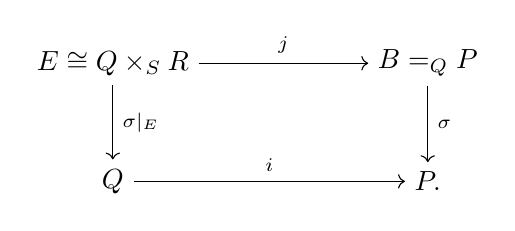
\begin{tikzpicture}[auto]
    \node (B) at (0,1.5) {\(E \cong Q\times_SR\)};
    \node (A) at (0,0) {\(Q\)};
    \node (B') at (4,1.5) {\(B = \Bl_QP\)};
    \node (A') at (4,0) {\(P. \)};
    \draw[->] (B) to node{\scriptsize \(\sigma|_E\)} (A);
    \draw[->] (B) to node{\scriptsize \(j\)} (B');
    \draw[->] (B') to node{\scriptsize \(\sigma\)} (A');
    \draw[->] (A) to node{\scriptsize \(i\)} (A');
  \end{tikzpicture}
  \]
  \HereEndTikz
  \(E\)のイデアル層 (=blow-upのトートロジカル束)
  を\(\mcI_E\)または\(\OO{B/P}(1)\)と書く。
\end{setting*}


自然な同型\(\mcI \cong \sigma_*(\OO{B/P}(1))\)から、自然に
\[
\mcI(1) \cong \sigma_*(\OO{B/P}(1)\otimes \sigma^*(\OO{P/S}(1)))
\]
となることがわかる。
よって、\(\mcK_P\to \OO{P/S}(1)\)の\(B\)への基底変換
\(\mcK_B\to \sigma^*(\OO{P/S}(1))\)は
\(\OO{B/P}(1)\otimes \sigma^*(\OO{P/S}(1)) \subset \sigma^*(\OO{P/S}(1))\)
を一意的に経由する。

\begin{lem}
  \(\mcK_B\to \OO{B/P}(1)\otimes \sigma^*(\OO{P/S}(1))\)は全射である。
\end{lem}

\begin{proof}
  \(\mcK_P\to \mcI(1)\)が全射であることと、
  \(\sigma\)が\(E\)の外では同型射であることから、
  \(E\)の外では全射である。
  よって\(E\)上で全射であることを示せば良い。
  \(E\)へと基底変換する。
  \((\OO{B/P}(1) \otimes \sigma^*(\OO{P/S}(1)))|_E
  \cong \OO{E/Q}(1) \otimes \sigma|_E^*(\OO{Q/S}(1))\)
  であるから、
  \(\mcK_B\to \OO{B/P}(1)\otimes \sigma^*(\OO{P/S}(1))\)
  の\(E\)への制限は
  \[
  \mcK_E\to \OO{E/Q}(1) \otimes \sigma|_E^*\OO{Q/S}(1)
  \]
  となる。
  \(\mcK_E\to \OO{E/Q}(1) \otimes \sigma|_E^*\OO{Q/S}(1)\)は
  \(\mcK_P\to \mcI(1)\)という全射から自然に得られる射であるから、
  \[
  \mcK_E \to \sigma|_E^*(\mcI/\mcI^2(1)) \to
  \OO{E/Q}(1) \otimes \sigma|_E^*(\OO{Q/S}(1))
  \]
  と分解する。
  ここで\(\mcK_E \to \sigma|_E^*(\mcI/\mcI^2(1))\)は同型射の引き戻しなので同型であり、
  \(\sigma|_E^*(\mcI/\mcI^2(1)) \to
  \OO{E/Q}(1) \otimes \sigma|_E^*\OO{Q/S}(1)\)は
  \(E\cong \P_Q(\mcI/\mcI^2)\)であることにより得られる全射
  \(\sigma|_E^*(\mcI/\mcI^2)\to \OO{E/Q}(1)\)に
  直線束\(\sigma|_E^*(\OO{Q/S}(1))\)をテンソルしたものであるから全射である。
  以上より\(\mcK_E\to \OO{E/Q}(1) \otimes \sigma|_E^*(\OO{Q/S}(1))\)は全射であることがわかり、
  証明が完了する。
\end{proof}


\(\OO{B/P}(1)\otimes \sigma^*(\OO{P/S}(1))\)は直線束なので、
全射\(\mcK_B\to \OO{B/P}(1)\otimes \sigma^*(\OO{P/S}(1))\)
は射\(\varphi:B\to R\)を引き起こす。
\(\sigma, \varphi\)により出る射\(B\to P\times_S R\)と合わせて、
以下の図式ができる (以下のように射に名前をつけておく):
\HereBeginTikz
\[
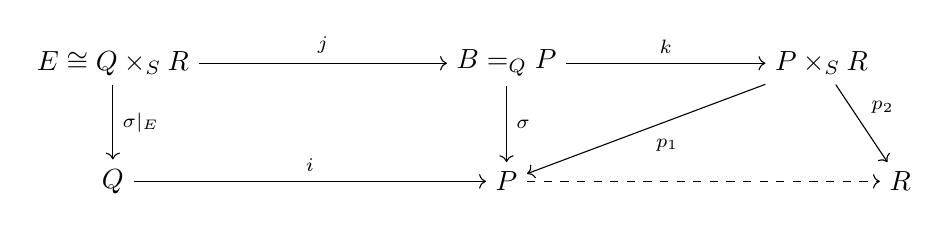
\begin{tikzpicture}[auto]
  \node (B) at (0,1.5) {\(E \cong Q\times_SR\)};
  \node (A) at (0,0) {\(Q\)};
  \node (B') at (5,1.5) {\(B = \Bl_QP\)};
  \node (A') at (5,0) {\(P\)};
  \node (B'') at (9,1.5) {\(P\times_SR\)};
  \node (A'') at (10,0) {\(R\)};
  \draw[->] (B) to node{\scriptsize \(\sigma|_E\)} (A);
  \draw[->] (B) to node{\scriptsize \(j\)} (B');
  \draw[->] (B') to node{\scriptsize \(\sigma\)} (A');
  \draw[->] (A) to node{\scriptsize \(i\)} (A');
  \draw[->] (B') to node{\scriptsize \(k\)} (B'');
  \draw[->] (B'') to node{\scriptsize \(p_1\)} (A');
  \draw[->] (B'') to node{\scriptsize \(p_2\)} (A'');
  \draw[->,dashed] (A') to (A'');
\end{tikzpicture}
\]
\HereEndTikz
右下の (有理写像\(P\dto R\)によってできる) 三角形以外は可換である。
\(k\)は\(B\)上の全射
\(\mcK_B\to \OO{B/P}(1)\otimes \sigma^*(\OO{P/S}(1))\)
により得られるが、
この全射の\(E\)への制限は
\(\sigma|_E^*(\mcI/\mcI^2)\to \OO{E/Q}(1)\)
を\(1\)回捻ったものであったから、
\(k\circ j\)は\(i:Q\to P\)の\(p_1:P\times_SR \to P\)による基底変換そのものである。
特に、\(k\circ j\)は閉埋め込みである。
従って\(k\)は閉部分集合の上への同相である。
また、\(\OO{P\times_SR}\to k_*\OB\)は\(p_1^{-1}(Q)\)
(つまり\(k\circ j\)の像、つまり\(E\)) の外で全射であり、
射の列
\(\OO{P\times_SR}\to k_*\OB \to k_*j_*\OE\)
の合成も全射である。
さらに\(k_*\OB \to k_*j_*\OE\)は全射のAffine射によるpushであるから全射である。
以上から、\(\OO{P\times_SR}\to k_*\OB\)の\(E\)への制限は全射である。
よって\(k\)は閉埋め込みとなる。

構成から、\(\varphi\)の各fiberは
次元\(\rank(\mcF)\)の射影空間となる。
\(B\)が\(R\)上の射影束としてどのような構造を持つかを決定する。


\begin{thm}\label{thm: main}
  \(R\)上のトートロジカルな全射\(\mcK_R\to \OO{R/S}(1)\)により、射
  \[
  \Ext^1_{\OR}(\mcF_R,\mcK_R) \to
  \Ext^1_{\OR}(\mcF_R,\OO{R/S}(1))
  \]
  を得る。
  与えられたはじめの完全列のうつる先を
  \[
  \begin{CD}
    0 @>>> \OO{R/S}(1) @>>> \mcG @>>> \mcF_R @>>> 0
  \end{CD}
  \]
  とする。
  このとき、\(B\)は\(R\)上の射影束\(\P_R(\mcG)\)と同型である。
\end{thm}


\begin{proof}
  まず\(\mcG\)の構成は\(\mcG\cong \mcE_R/(\ker (\mcK_R\to \OO{R/S}(1)))\)であり、
  \begin{equation}\label{eq: exace over R}
    \begin{CD}
      0 @>>> \mcK_R @>>> \mcE_R @>>> \mcF_R @>>> 0 \\
      @. @VVV @VVV @| @.\\
      0 @>>> \OO{R/S}(1) @>>> \mcG @>>> \mcF_R @>>> 0
    \end{CD}
    \tag{\(\ddagger\)}
  \end{equation}
  という\(R\)上の完全列の間の射が得られることに注意しておく。
  全射\(\mcG\to \mcF_R\)により、閉埋め込み
  \(E\cong Q\times_SR\to \P_R(\mcG)\)が得られ、
  全射\(\mcE_R\to \mcG\)により、閉埋め込み
  \(h:\P_R(\mcG)\to P\times_SR\)が得られる。
  この二つの閉埋め込みの合成は、
  全射\(\mcE_R\to \mcF_R\)により得られる閉埋め込み、
  すなわち\(k\circ j:E\to P\times_SR\)に他ならない。

  \(k:B\to P\times_SR\)が
  閉埋め込み\(\P_R(\mcG)\to P\times_SR\)を経由することを示す。
  完全列の射\eqref{eq: exace over R}を\(\varphi\)で\(B\)上へ基底変換すると、
  完全列の射
  \[
  \begin{CD}
    0 @>>> \mcK_B @>>> \mcE_B @>>> \mcF_B @>>> 0 \\
    @. @VVV @VVV @| @. \\
    0 @>>> \varphi^*(\OO{R/S}(1)) @>>> \varphi^*\mcG @>>> \mcF_B @>>> 0
  \end{CD}
  \]
  を得る。
  \(\varphi\)は全射
  \(\mcK_B\to \OO{B/P}(1)\otimes \sigma^*(\OO{P/S}(1))\)
  により引き起こされたものであるから、自然に
  \[
  \varphi^*(\OO{R/S}(1))\cong \OO{B/P}(1)\otimes \sigma^*(\OO{P/S}(1))
  \]
  となる。
  また、\(B\)上の完全列の射
  \[
  \begin{CD}
    0 @>>> \mcK_B @>>> \mcE_B @>>> \mcF_B @>>> 0 \\
    @. @VVV @VVV @VVV @.\\
    0 @>>> \OO{B/P}(1)\otimes \sigma^*(\OO{P/S}(1)) @>>>
    \sigma^*(\OO{P/S}(1)) @>>> j_*(\OO{E/Q}(1)) @>>> 0
  \end{CD}
  \]
  から、
  \(\ker(\mcE_B\to \varphi^*\mcG)\subset
  \ker(\mcE_B\to \sigma^*(\OO{P/S}(1)))\)
  がわかり、全射\(\varphi^*\mcG\to \sigma^*(\OO{P/S}(1))\)を得る。
  全射\(\varphi^*\mcG\to \sigma^*(\OO{P/S}(1))\)
  が引き起こす射を\(f:B\to \P_R(\mcG)\)と置く。
  自然な同型
  \[
  \sigma^*(\OO{P/S}(1)) = k^*p_1^*(\OO{P/S}(1))\cong k^*(\OO{P\times_SR/R}(1))
  \]
  と全射\(\varphi^*\mcG\to \sigma^*(\OO{P/S}(1))\)の構成から、図式
  \[
  \begin{CD}
    \mcE_B @>>> k^*\OO{P\times_SR/R}(1) \\
    @VVV @VV\cong V \\
    \varphi^*\mcG @>>> \sigma^*\OO{P/S}(1)
  \end{CD}
  \]
  は可換であり、従って\(h\circ f = k\)となる。
  特に\(f\)は閉埋め込みである。

  \(s\dfn f\circ j:E \to \P_R(\mcG)\)と置く。
  \(s\)は\(R\)上の層の全射\(\mcG_R\to \mcF_R\)により引き起こされた射である。
  \(k\circ j:E\to P\times_SR\)が\(i:Q\to P\)の基底変換であることに注意すれば、
  \((p_1\circ h)^*\mcI\to \OO{\P_R(\mcG)}\)の像は
  \(s\)のイデアル層と一致することがわかる。
  一方、\(\mcG_R\to \mcF_R\)の核は直線束であるから、
  \(s\)のイデアル層は直線束である。
  \(B\)は\(Q\)のイデアル層\(\mcI\)による\(P\)の爆発であるから、
  射\(g:\P_R(\mcG)\to B\)が存在して\(\sigma\circ g = p_1\circ h\)となる。
  また、
  \[
  g^*f^*\OO{\P_R(\mcG)/R}(1)\cong g^*\sigma^*\OO{B/P}(1)\cong
  h^*p_1^*\OO{B/P}(1)\cong h^*\OO{P\times_SR/R}(1)\cong \OO{\P_R(\mcG)/R}(1)
  \]
  であるから、\(f\circ g\)は同型射であり、
  特に\(f\)は全射となる。
  \(f\)は閉埋め込みだったので、\(f\)は同型射であることがわかり、
  以上で\(B\cong \P_R(\mcG)\)がわかる。
\end{proof}




\begin{cor}\label{cor: main}
  \(V\to W\)を有限次元\(k\)-線形空間の全射、
  \(K\)をその核とし、
  \(\P(V)\)の\(\P(W)\)に沿った爆発を\(B\)と置くと、
  \(B\cong \P_{\P(K)}(\OO{\P(K)}(1)\oplus W_{\P(K)})\)となる。
\end{cor}

\begin{proof}
  \(\Ext^1_{\OO{\P(K)}}(W_{\P(K)}, \OO{\P(K)}(1))
  \cong H^1(\P(K), \OO{\P(K)}(1))\otimes_kW^{\vee} = 0\)であるから、
  完全列
  \[
  \begin{CD}
    0 @>>> \OO{\P(K)}(1) @>>> \mcG @>>> W_{\P(K)} @>>> 0
  \end{CD}
  \]
  は分裂する。
\end{proof}


\begin{cor}
  \(\P^n\)の一点爆発は
  \(\P_{\P^{n-1}}(\OO{\P^{n-1}}\oplus \OO{\P^{n-1}}(1))\)
  と同型である。
\end{cor}


\begin{cor}
  \(V\)を次元\(r+1\)の\(k\)-線形空間、
  \(0<s<r\)を自然数、
  \(\mathbb{G}(V,s+1)\)を次元\(s\)の\(\P(V)\)の平面をパラメタライズするグラスマン多様体、
  \[
  p:V_{\mathbb{G}(V,s+1)}\to \mcU
  \]
  をランク\(s+1\)の局所自由層へのトートロジカルな全射、
  \(\mcK \dfn \ker(p)\)を\(p\)の核 (これはランク\(r-s\)である)、
  \(\P_{\mathbb{G}(V,s+1)}(\mcU)\subset \mathbb{G}(V,s+1)\times \P(V)\)を
  \(\mathbb{G}(V,s+1)\)でパラメーター付けられた
  \(\P(V)\)の次元\(s\)の\(\P(V)\)の平面の普遍的な族
  (incidence variety) とする。
  \(\mathbb{G}(V,s+1)\times \P(V)\)を
  \(\P_{\mathbb{G}(V,s+1)}(\mcU)\)に沿って爆発した多様体を
  \(B\)と置くと、
  \(B\)は\(\P_{\mathbb{G}(V,s+1)}(\mcK)\)上の\(\P^{s+1}\)-束である。
\end{cor}


\begin{cor}
  \(V\)を\(k\)-線形空間、
  \(\Delta\subset \P(V)\times \P(V)\)を対角集合、
  \(B\)を\(\P(V)\times \P(V)\)の\(\Delta\)に沿った爆発とすると、
  \(B\)は\(\P_{\P(V)}(\Omega_{\P(V)})\)上の\(\P^1\)-束である。
\end{cor}




\begin{thebibliography}{9}
  \bibitem[Ha]{Ha}
  R.Hartshorne,
  \textit{Algebraic Geometry}.
  Springer-Verlag, New Tork, 1977. Graduate Text in Mathematics, No. 52.
\end{thebibliography}


\end{document}
